% !TEX TS-program = XeLaTeX
% use the following command:
% all document files must be coded in UTF-8
\documentclass[portuguese]{textolivre}
% build HTML with: make4ht -e build.lua -c textolivre.cfg -x -u article "fn-in,svg,pic-align"

\journalname{Texto Livre}
\thevolume{18}
%\thenumber{1} % old template
\theyear{2025}
\receiveddate{\DTMdisplaydate{2025}{4}{15}{-1}} % YYYY MM DD
\accepteddate{\DTMdisplaydate{2025}{6}{14}{-1}}
\publisheddate{\DTMdisplaydate{2025}{9}{10}{-1}}
\corrauthor{Geilson Fernandes de Oliveira}
\articledoi{10.1590/1983-3652.2025.58661}
%\articleid{NNNN} % if the article ID is not the last 5 numbers of its DOI, provide it using \articleid{} commmand 
% list of available sesscions in the journal: articles, dossier, reports, essays, reviews, interviews, editorial
\articlesessionname{articles}
\runningauthor{Oliveira et al.} 
%\editorname{Leonardo Araújo} % old template
\sectioneditorname{Daniervelin Pereira}
\layouteditorname{Leonado Araújo}

\title{Emoções e mudanças climáticas no Instagram: um estudo em contexto brasileiro}
\othertitle{Emotions and climate change on instagram: a study in the Brazilian context}
% if there is a third language title, add here:
%\othertitle{Artikelvorlage zur Einreichung beim Texto Livre Journal}

\author[1,2]{Geilson Fernandes de Oliveira~\orcid{0000-0002-3278-4044}\thanks{Email: \href{mailto:geilson.fernandes@gmail.com}{geilson.fernandes@gmail.com}}}
\author[2]{Luisa Massarani~\orcid{0000-0002-5710-7242}\thanks{Email: \href{mailto:luisa.massarani@fiocruz.br}{luisa.massarani@fiocruz.br}}}
\author[2]{Graziele Scalfi~\orcid{0000-0002-1417-1287}\thanks{Email: \href{mailto:graziscalfi@gmail.com}{graziscalfi@gmail.com}}}
\author[3]{Marcelo Alves dos Santos Junior~\orcid{0000-0003-4995-6612}\thanks{Email: \href{mailto:marcelo\_alves@puc-rio.br}{marcelo\_alves@puc-rio.br}}}
\author[4,2]{Thaiane Oliveira~\orcid{0000-0002-8588-3548}\thanks{Email: \href{mailto:thaianeoliveira@id.uff.br}{thaianeoliveira@id.uff.br}}}
\affil[1]{Universidade do Estado da Bahia, Juazeiro, BA, Brasil.}
\affil[2]{Fundação Oswaldo Cruz, Instituto Nacional de Comunicação Pública da Ciência e Tecnologia (INCT-CPCT), Rio de Janeiro, RJ, Brasil.}
\affil[3]{Pontifícia Universidade Católica do Rio de Janeiro, Rio de Janeiro, RJ, Brasil.}
\affil[4]{Universidade Federal Fluminense, Niterói, RJ, Brasil.}

\addbibresource{article.bib}
% use biber instead of bibtex
% $ biber article

% used to create dummy text for the template file
\definecolor{dark-gray}{gray}{0.35} % color used to display dummy texts
\usepackage{lipsum}
\SetLipsumParListSurrounders{\colorlet{oldcolor}{.}\color{dark-gray}}{\color{oldcolor}}

% used here only to provide the XeLaTeX and BibTeX logos
\usepackage{hologo}

% if you use multirows in a table, include the multirow package
\usepackage{multirow}

% provides sidewaysfigure environment
\usepackage{rotating}

% CUSTOM EPIGRAPH - BEGIN 
%%% https://tex.stackexchange.com/questions/193178/specific-epigraph-style
\usepackage{epigraph}
\renewcommand\textflush{flushright}
\makeatletter
\newlength\epitextskip
\pretocmd{\@epitext}{\em}{}{}
\apptocmd{\@epitext}{\em}{}{}
\patchcmd{\epigraph}{\@epitext{#1}\\}{\@epitext{#1}\\[\epitextskip]}{}{}
\makeatother
\setlength\epigraphrule{0pt}
\setlength\epitextskip{0.5ex}
\setlength\epigraphwidth{.7\textwidth}
% CUSTOM EPIGRAPH - END

% to use IPA symbols in unicode add
%\usepackage{fontspec}
%\newfontfamily\ipafont{CMU Serif}
%\newcommand{\ipa}[1]{{\ipafont #1}}
% and in the text you may use the \ipa{...} command passing the symbols in unicode

% LANGUAGE - BEGIN
% ARABIC
% for languages that use special fonts, you must provide the typeface that will be used
% \setotherlanguage{arabic}
% \newfontfamily\arabicfont[Script=Arabic]{Amiri}
% \newfontfamily\arabicfontsf[Script=Arabic]{Amiri}
% \newfontfamily\arabicfonttt[Script=Arabic]{Amiri}
%
% in the article, to add arabic text use: \textlang{arabic}{ ... }
%
% RUSSIAN
% for russian text we also need to define fonts with support for Cyrillic script
% \usepackage{fontspec}
% \setotherlanguage{russian}
% \newfontfamily\cyrillicfont{Times New Roman}
% \newfontfamily\cyrillicfontsf{Times New Roman}[Script=Cyrillic]
% \newfontfamily\cyrillicfonttt{Times New Roman}[Script=Cyrillic]
%
% in the text use \begin{russian} ... \end{russian}
% LANGUAGE - END

% EMOJIS - BEGIN
% to use emoticons in your manuscript
% https://stackoverflow.com/questions/190145/how-to-insert-emoticons-in-latex/57076064
% using font Symbola, which has full support
% the font may be downloaded at:
% https://dn-works.com/ufas/
% add to preamble:
\newfontfamily\Symbola{Symbola}
% in the text use:
% {\Symbola }
% EMOJIS - END

% LABEL REFERENCE TO DESCRIPTIVE LIST - BEGIN
% reference itens in a descriptive list using their labels instead of numbers
% insert the code below in the preambule:
%\makeatletter
%\let\orgdescriptionlabel\descriptionlabel
%\renewcommand*{\descriptionlabel}[1]{%
%  \let\orglabel\label
%  \let\label\@gobble
%  \phantomsection
%  \edef\@currentlabel{#1\unskip}%
%  \let\label\orglabel
%  \orgdescriptionlabel{#1}%
%}
%\makeatother
%
% in your document, use as illustraded here:
%\begin{description}
%  \item[first\label{itm1}] this is only an example;
%  % ...  add more items
%\end{description}
% LABEL REFERENCE TO DESCRIPTIVE LIST - END


% add line numbers for submission
%\usepackage{lineno}
%\linenumbers

\begin{document}
\maketitle

\begin{polyabstract}
\begin{abstract}
Entendidas como as transformações de longo prazo nos padrões de temperatura e clima, as mudanças climáticas ganham cada vez mais espaço no debate público. Neste artigo, objetivamos analisar as emoções expressas nos conteúdos brasileiros sobre o tema no Instagram. Partimos de uma amostra aleatória construída a partir de 1.067 \textit{posts} sobre o tópico entre 2021 e 2022, coletada por meio do Crowdtangle. A identificação das emoções foi realizada a partir dos descritores da \textit{Human-Machine Interaction Network on Emotion} e do \textit{Core Affect Model}. Teoricamente, a investigação se situa em um campo multidisciplinar, compreendendo as discussões acerca das mudanças climáticas, estudo das emoções e redes sociais da internet. Como resultado, observou-se um número relativamente pequeno de publicações com expressão de emoções no \textit{corpus} (18,5\%). Destas, verificou-se a prevalência de emoções negativas (61,2\%), como preocupação (23,7\%) e desaprovação (20,7\%). Em menor quantidade, emoções positivas (38,8\%) como interesse (18,9\%) e esperança (6,6\%) também foram expressas. As análises apontam a necessidade de reflexões sobre as emoções identificadas, que de diferentes maneiras indicam um viés de atenção sobre as mudanças climáticas e possibilidades para lidar com o seu avanço.

\keywords{Mudanças climáticas \sep Emoções \sep Instagram \sep Brasil}
\end{abstract}

\begin{english}
\begin{abstract}
Understood as long-term transformations in temperature and climate patterns, climate change is gaining increasing attention in public debates. In this article, we aim to analyze the emotions expressed in Brazilian content on Instagram regarding this topic. We started with a random sample of 1,067 posts on the subject between 2021 and 2022, collected through Crowdtangle. The identification of emotions was based on the descriptors from the Human-Machine Interaction Network on Emotion and the Core Affect Model. Theoretically, the research is situated in a multidisciplinary field, encompassing discussions about climate change, the study of emotions and social networks on the internet. As a result, a relatively small number of posts expressing emotions was observed in the corpus (18.5\%). Among these, the prevalence of negative emotions (61.2\%) was noted, with concern (23.7\%) and disapproval (20.7\%) standing out. In smaller quantities, positive emotions (38.8\%) such as interest (18.9\%) and hope (6.6\%) were also expressed. The analyses highlight the need for reflection on the identified emotions, which in different ways indicate an attention bias towards climate change and possibilities for addressing its advancement.

\keywords{Climate change \sep Emotions \sep Instagram \sep Brazil}
\end{abstract}
\end{english}
% if there is another abstract, insert it here using the same scheme
\end{polyabstract}

\section{Introdução}\label{sec-intro}
Nos últimos anos, diferentes expressões como efeito estufa, aquecimento global, buraco na camada de ozônio, mudanças climáticas, entre outras, têm sido utilizadas para se referir às transformações de longo prazo nos padrões de temperatura e clima, provocadas, especialmente, por causa das ações humanas, entre elas o crescimento exponencial de emissões de gases advindos da queima de combustíveis fósseis e dos processos de exploração e desmatamento das florestas. A recorrência dessas discussões tem ocupado novos espaços na esfera pública e chamado atenção em se tratando de promoção de políticas que possam reduzir as suas consequências, o que é visto como necessário diante de acontecimentos cada vez mais frequentes indicados como desdobramentos de todo esse processo (como secas, enchentes e alagamentos, derretimento de geleiras, aumento do nível do mar, por exemplo).

Nesse contexto, há uma crescente produção discursiva acerca do fenômeno das mudanças climáticas, abordando, de maneira geral, as suas causas e seus desdobramentos para a vida em sociedade. Nas redes sociais da internet, espaços utilizados de forma extensiva para a promoção de discussões públicas por parte de diferentes atores e grupos, a questão das mudanças climáticas também tem se tornado tema frequente, principalmente quando da ocorrência de acontecimentos que são compreendidos como efeitos desses processos \cite{araujo2021brumadinho}. Além disso, iniciativas que buscam promover ações de combate às mudanças climáticas também têm feito uso dessas plataformas para difundir suas ideias, construir comunidades de pertencimento e se aproximar de novos públicos \cite{balbe2016mudancas}.

Considerando essas discussões, neste artigo, investigamos a circulação de conteúdos acerca das mudanças climáticas no contexto brasileiro na rede social da internet Instagram, que tem se destacado no Brasil tanto em termos de número de usuários \cite{bianchi2024socialmedia}, como também no que concerne à sua vultosa produção de conteúdos e consumo \cite{newman2023reuters}, buscando refletir, especialmente, sobre as emoções que são mobilizadas a partir das discussões sobre as mudanças climáticas. A proposta de se investigar a expressão das emoções referentes aos conteúdos sobre essa temática se dá levando em conta a necessidade de identificar como o assunto tem sido percebido e interpretado pelo público a partir de uma dimensão muitas vezes pouco explorada, partindo-se do pressuposto de que as emoções são fenômenos complexos \cite{barrett2017emotions} por meio dos quais podemos melhor compreender atitudes, interesses e percepções públicas sobre a realidade \cite{fernandesdeoliveira2023vacina}.

De acordo com \textcite{newman2023reuters}, no Brasil, o Instagram é utilizado por 39\% da população como fonte de informação, número que cresce significativamente quando se analisa o seu uso para fins gerais, como produção de conteúdo e entretenimento, chegando aos 63\%. Em 2023, o Instagram foi a segunda rede social mais utilizada pelos brasileiros, atrás apenas do WhatsApp \cite{bianchi2024socialmedia}. Nesse sentido, trata-se de uma plataforma com amplo uso, a partir da qual a vida social e seus processos são mediados, contemplando, dentre as suas discussões, o tema das mudanças climáticas.

Assim entendido, partimos das seguintes questões de pesquisa: 1) Quais emoções estão articuladas às postagens produzidas e publicadas sobre mudanças climáticas no Instagram, considerando o cenário brasileiro? 2) Quais são as emoções expressas de maneira mais frequente nos conteúdos sobre o tema? 3) Que tópicos de discussões, associados às mudanças climáticas, mais mobilizam emoções? Com o objetivo de responder essas perguntas, selecionamos como recorte uma amostra aleatória construída a partir de 1.067 \textit{posts} públicos que abordam o tema das mudanças climáticas no Instagram, levando em conta os conteúdos produzidos no contexto brasileiro entre os anos de 2021 e 2022, coletada por meio da interface gráfica do Crowdtangle. Teoricamente, a investigação se situa em um campo multidisciplinar, compreendendo as discussões acerca das mudanças climáticas, estudo das emoções e redes sociais da internet.

A investigação proposta se mostra como atual e relevante, considerando a necessidade de se entender como a questão das mudanças climáticas vem sendo pautada, assim como sobre quais emoções estão associadas à problemática, haja vista que fatores subjacentes à compreensão pública sobre as alterações climáticas têm se tornado importante área de investigação \cite{lu2015incidental}. A reflexão sobre as emoções, nessa perspectiva, é vista como fonte valiosa de informação devido ao fato de se referir a uma discussão que envolve transformações cada vez mais frequentes e com maior incidência em diferentes contextos, podendo contribuir para a compreensão dos modos de leitura e interpretação acerca das mudanças climáticas por parte dos públicos envolvidos no debate.

\section{Mudanças climáticas}\label{sec-normas}
Apesar de não ser uma discussão inteiramente nova, a temática das mudanças climáticas ganhou impulso no campo acadêmico, compreendendo a sua abordagem a partir de diferentes áreas, principalmente, a partir do final dos anos 1980 e início de 1990 \cite{chakrabarty2009climate}, vindo a se tornar uma preocupação efetivamente pública somente a partir dos anos 2000 \cite{fleury2019mudancas}.

Mais recentemente, porém, tanto a questão das mudanças climáticas quanto as discussões sobre os modelos de desenvolvimento econômico vêm sendo problematizadas, especialmente, diante de acontecimentos que têm se apresentando como desdobramentos da intensa ação humana em relação à natureza \cite{conti2011consideracoes,artaxo2020emergencias}. Sobre esse aspecto, no que diz respeito especificamente ao Brasil, o Primeiro Relatório de Avaliação Nacional do Painel Brasileiro de Mudanças Climáticas \cite{ambrizzi2014pbmc}, responsável por reunir dados sobre a temática e fornecer projeções para o clima a partir dos diferentes biomas, indicou que mudanças importantes devem ocorrer ainda neste século.

Essas constatações, que são também fornecidas por diferentes cientistas, apontam para as mudanças climáticas como um problema que repercute nas condições climatológicas de todo o planeta \cite{flores2018emociones,cartea2009comunicar}. Essa perspectiva tem circulado a partir dos meios informativos e noticiosos, sendo entendida pelos seus públicos a partir de percepções que transitam entre o descrédito, negação e preocupação \cite{almeida2019sociologia} até a esperança depositada por aqueles que acreditam, a partir de suas ações, poder desacelerar as mudanças já em curso.

Nessa esteira, pesquisas recentes demonstram que a percepção de que as mudanças climáticas são um problema grave vem aumentando. É o que tem acontecido no Brasil, de acordo com pesquisa desenvolvida pelo Instituto Tecnologia e Sociedade (ITS Rio) em parceria com o Ipec (Inteligência em Pesquisa e Consultoria), ao apontar que 94\% dos brasileiros acreditavam em 2022 que o aquecimento global está acontecendo, número maior do que aquele apresentado em 2020, quando 92\% indicaram essa visão. Pesquisa mais recente, divulgada pelo Centro de Gestão e Estudos Estratégicos \cite{cgee2024percepcao} corrobora esses dados, apontando que em relação à percepção sobre mudanças climáticas, 95,4\% dos brasileiros entrevistados afirmam que elas estão acontecendo. Desse total, 78,2\% acreditam que esse fenômeno é causado principalmente pela ação humana, o que é considerado por 60,5\% como um grave perigo.

Em se tratando dos campos de estudo da Comunicação e da Mídia, as mudanças climáticas têm sido investigadas a partir de diferentes perspectivas, compreendendo desde pesquisas sobre a cobertura em torno da temática \cite{loose2017jornalismo,rodas2017midia}, até casos com análises mais específicas, focadas em acontecimentos relativos aos desastres ambientais \cite{bueno2017cobertura,mancuso2010enchentes}, contemplando, ainda, reflexões sobre as representações e enquadramentos acerca das mudanças climáticas \cite{campos2021desmatamento}, o papel da comunicação nesses processos \cite{rodas2017midia}, os riscos da desinformação no que concerne à temática \cite{treen2020misinformation,santini2022negacionismo}, debates acerca da questão nas redes sociais \cite{evangelista2024narrativas,basch2021tiktok,balbe2016mudancas}, bem como, estudos que buscam refletir sobre as emoções como elementos constitutivos dos conteúdos produzidos \cite{brosch2021affect,roeser2012risk,lu2015incidental}.

De maneira geral, a maior parte desses estudos reflete e aponta para o papel e a importância da Comunicação e da Mídia na mediação dos acontecimentos que envolvem as mudanças climáticas, considerando tanto a sua produção de sentidos para a compreensão da temática por parte do público, como também a sua responsabilidade, levando em conta o teor sensível de seus conteúdos. Dessa forma, apontam para os cuidados que devem ser observados quando do tratamento da situação, considerando seus riscos, projeções e controvérsias \cite{rodas2017midia}.

\subsection{Mudanças climáticas, emoções e redes sociais}\label{sec-conduta}
Uma variedade de reflexões tem sido desenvolvida com vistas a problematizar o papel das emoções em relação aos conteúdos sobre mudanças climáticas. Isto porque as emoções vêm sendo vistas como elementos que possuem fortes ligações com os processos cognitivos, além de constitutivas dos processos de tomada de decisões, fornecendo informações e avaliações importantes em termos de comportamentos relativos a eventos que têm se constituído como preocupações globais \cite{brosch2021affect,roeser2012risk}. Nessa perspectiva, as emoções, muitas vezes associadas à irracionalidade, são compreendidas como fenômenos cognitivos, racionais e reflexivos \cite{lerner2015emotion,brosch2013impact}.

A compreensão dos aspectos inerentes às discussões públicas sobre mudanças climáticas, levando em conta as emoções que são agenciadas e expressas, nesse sentido, se torna uma relevante área de investigação. Acerca dessa questão, de forma crescente, pesquisas têm apontado que as emoções desempenham uma função importante no que diz respeito à orientação e tomada de decisão em torno das formas como o público decodifica e reage aos conteúdos relativos às mudanças climáticas \cite{lu2015incidental,salama2018role}.

Nessa perspectiva, a fim de compreender as relações entre emoções e mudanças climáticas, \textcite{harth2021affect} examinou a literatura recente em torno dessa discussão. Conforme o autor, os estudos identificados mostram que as emoções são fenômenos essenciais para o desenvolvimento de ações sobre as mudanças climáticas, seja em nível individual ou em grupo. Com efeito, as mudanças climáticas são percebidas como uma questão que envolve as emoções para além dos seus aspectos ambientais, sociais, culturais e políticos. Levando em conta essa concepção, pesquisadores têm problematizado como os comunicadores podem usar as emoções para apoiar ou motivar ações que possam frear as mudanças climáticas \cite{salama2018role,roeser2012risk,brosch2021affect}.

Entre os resultados dessas pesquisas, foi verificado que as emoções podem ser um dos aspectos potenciais no sentido de favorecer a relação entre a comunicação sobre as mudanças climáticas, percepção do público e mudança de comportamento \cite{salama2018role,chapman2017reassessing}. Isto porque as emoções que as pessoas experimentam, no que se refere às mudanças climáticas, são vistas como preditoras da percepção de risco e mudanças de comportamento \cite{brosch2021affect}. Entretanto, vale salientar que ao mesmo tempo em que as emoções podem ser aliadas, a depender da forma como são exploradas, também podem se constituir como barreiras, no sentido de que uma ênfase em determinadas emoções, como a culpa, mobilizada a partir da responsabilização voltada para a sociedade, por exemplo, pode afastar o público, resultando em efeitos negativos \cite{harth2021affect}. Se tem, dessa forma, o entendimento de que as emoções não devem ser utilizadas ou vistas nesses processos de forma não planejada ou como simples instrumentos, pois dizem respeito a um fenômeno complexo, não havendo uma abordagem com um único modelo \cite{chapman2017reassessing}, se considerando questões relativas às temáticas, contextos e públicos relacionados.

Além das análises voltadas para o papel das emoções nos processos de comunicação sobre mudanças climáticas, outros estudos têm explorado a relação entre as representações produzidas em torno das alterações do clima e as emoções mobilizadas nesses conteúdos, bem como expressas pelos públicos que os consomem. \textcite{feldman2017hope} testaram, por exemplo, como os efeitos das imagens e textos que abordam as causas e impactos das alterações climáticas podem se constituir como base para ações voltadas ao enfrentamento das mudanças no clima. Suas conclusões indicaram que as imagens e textos noticiosos e informativos pautados na temática do clima podem aumentar a esperança, diminuir o medo e a raiva, emoções que são produzidas e mobilizadas a partir dos processos de representação.

\textcite{flores2018emociones}, por sua vez, investigaram os principais componentes emocionais mobilizados a partir das representações sociais das mudanças climáticas juntamente a um grupo de estudantes no México. Como resultado, se observou com maior frequência a expressão de emoções negativas por parte dos estudantes, com ênfase na indignação, tristeza, medo, entre outras. Ressalta-se que, apesar de negativas, essas emoções indicavam ao mesmo tempo um viés de protesto e ação, como no caso da indignação, tendo em vista a sua motivação a partir da ausência de ações concretas por parte de figuras políticas para lidar com a situação \cite{flores2018emociones}. Esses achados evidenciam o quanto as emoções se constituem como componentes relevantes das representações sociais e das discussões sobre mudanças climáticas.

Outros estudos, ainda, têm abordado a temática a partir da sua circulação nas redes sociais, vistas como ferramentas importantes para se compreender a opinião pública sobre diferentes assuntos. \textcite{basch2021tiktok,sun2024tiktok} investigaram a questão das mudanças climáticas na plataforma de vídeos TikTok. O primeiro estudo buscou descrever os conteúdos em língua inglesa relacionado ao assunto a partir da \textit{hashtag} \textit{\#climatechange}, apontando, entre os seus resultados, para a necessidade de presença de profissionais credíveis para tratar do assunto de maneira mais sólida, já que foi identificada uma produção com pouca sustentação científica, o que pode contribuir para processos de desinformação e percepções negativas \cite{basch2021tiktok}.

\textcite{sun2024tiktok}, a seu turno, delinearam as representações de notícias e desastres relacionados ao clima a partir de cinquenta contas do TikTok focadas no assunto. Os resultados se assemelham aos do estudo de \textcite{basch2021tiktok}, já que se observa que a produção de conteúdos realizada por influenciadores da internet possui mais impacto na divulgação de conteúdos sobre o clima do que cientistas ou governo, o que é verificado a partir da quantidade de visualizações, comentários e compartilhamentos dos conteúdos. Logo, aponta-se para a necessidade da presença de especialistas para abordar o assunto, a fim de se construir informações com maior solidez e profundidade.

Articulando as investigações entre mudanças climáticas, emoções e redes sociais, ao analisar os conteúdos que abordam a questão do clima no Twitter (atual X) durante os anos de 2008 a 2014, \textcite{cody2015climate} apontam que a maioria dos \textit{posts} relacionados à palavra “clima” esteve associada a um sentido negativo, haja vista as repercussões negativas no que se refere aos desastres naturais. De acordo com a investigação, desastres naturais, mudanças climáticas e exploração dos bens naturais tendem a contribuir para uma diminuição de emoções positivas nos conteúdos examinados, ao passo em que eventos sobre o clima, novas discussões ou ideias pró-meio ambiente favorecem um aumento de emoções positivas.

Outra questão importante na abordagem sobre mudanças climáticas é observada na pesquisa de \textcite{haastrup2022personalising}, que analisou os perfis no Instagram de três personalidades diretamente envolvidas com as discussões sobre o clima na Dinamarca (um ativista, um influenciador e um político). Segundo o autor, o envolvimento afetivo dos atores em relação ao assunto das alterações do clima lhes confere autenticidade e confiança junto aos seus públicos.

No cenário brasileiro, ainda são escassas as pesquisas acerca da relação entre mudanças climáticas, emoções e redes sociais. Apesar disso, algumas investigações vêm sendo realizadas a esse respeito, como o trabalho de \textcite{balbe2020jornalismo}, que buscou mapear a partir de uma pesquisa bibliográfica o que já foi investigado sobre a relação entre o medo e as alterações climáticas na cobertura jornalística. Com efeito, constatou-se que ainda há poucas reflexões científicas sobre a questão, reforçando a necessidade de mais investigações empíricas, principalmente diante do aumento de conteúdos jornalísticos pautados em abordagens espetacularizadas e alarmistas, o que segundo as autoras pode ter efeitos diversos junto ao público, podendo, inclusive, promover a desmobilização em prol de ações favoráveis ao meio ambiente.

Em estudo sobre os debates em torno das mudanças climáticas durante a 21ª Conferência das Partes (COP21), tendo como recorte o Twitter (atual X), \textcite{balbe2017twitter} reforçam que as pesquisas sobre comunicação e mudanças climáticas no contexto das redes sociais são limitadas, sobretudo, em língua portuguesa. Além dessa constatação, as autoras indicaram como resultado da investigação que as mensagens mais populares sobre a COP21 na rede investigada não compreenderam, no geral, referências negacionistas sobre as mudanças climáticas, ainda que em alguns casos as mudanças no clima tenham sido identificadas como uma hipótese. A maioria das abordagens, ressaltam \textcite{balbe2017twitter}, compreendeu as consequências para o futuro, atribuindo expectativas positivas para a promoção de um acordo global, evidenciando um viés esperançoso e otimista em termos emocionais.

Já \textcite{evangelista2024narrativas} realizaram estudo exploratório sobre os discursos em circulação no TikTok sobre as mudanças climáticas no Brasil a partir dos 50 vídeos indicados pela plataforma como mais relevantes com a \textit{hashtag} \textit{\#mudancaclimatica}. Os resultados da pesquisa demonstraram a existência de um relativo consenso sobre a veracidade e gravidade das mudanças climáticas, apesar da complexidade da questão ser colocada em um segundo plano. Destaca-se, ainda, a presença de um tom alarmista nas narrativas construídas -- o que tende a atuar mais na promoção do medo do que contribuir em termos informativos --, bem como dificuldades na identificação das fontes e canais responsáveis pelas produções \cite{evangelista2024narrativas}. Ademais, destaca-se a presença, ainda que pequena, da responsabilização aos governos pelas alterações no clima, o que foi identificado em 11 dos vídeos examinados, com ênfase às críticas relativas à postura do ex-presidente do Brasil, Jair Messias Bolsonaro, fonte de desaprovação.

Como se pode observar, a questão das emoções nem sempre se constitui como o elemento central das pesquisas brasileiras citadas, havendo a necessidade de aprofundar a sua compreensão, principalmente nos conteúdos sobre mudanças climáticas produzidos nas redes sociais, espaços identificados como de ampla circulação de discussões sobre a temática, assim como ambiências favoráveis para as trocas comunicacionais mediadas pelas emoções e afetividade \cite{papacharissi2014affective,serrano2016internet}. Com vistas a contribuir com essa perspectiva é que nos propomos a analisar as emoções mobilizadas acerca das mudanças climáticas no contexto brasileiro na rede social Instagram.


\section{Procedimentos metodológicos}\label{sec-fmt-manuscrito}
\subsection{Coleta dos dados}
A coleta dos dados desta pesquisa foi realizada por meio da interface gráfica do Crowdtangle, compreendendo como palavras-chave para a busca e composição do \textit{corpus} os termos “mudança climática”, “mudanças climáticas”, “crise climática” e “aquecimento global” em conteúdos produzidos em perfis públicos do Instagram no Brasil entre 01 de janeiro de 2021 a 31 de dezembro de 2022, período selecionado levando em conta a posição complexa que o Brasil ocupava naquele momento, considerando-se as repercussões negativas acerca das políticas e ações do governo Federal em relação ao meio ambiente. Como resultado, foi coletado um total de 16.526 publicações.

Após esse processo, construímos uma amostra aleatória a partir de 1.067 \textit{posts}. O critério de aleatoriedade foi selecionado a fim de se produzir uma visão mais geral sobre o assunto, considerando que a escolha dos \textit{posts} com maior engajamento (curtidas, comentários e compartilhamentos) acabaria por apontar para uma carga emocional já delimitada, tendo em vista as questões relacionadas aos aspectos de circulação e preferência algorítmica \cite{berger2012viral} das plataformas de redes sociais.


\subsection{Identificação e classificação das emoções}\label{sec-formato}
Uma vez realizada a coleta e composição do \textit{corpus} da pesquisa, cada post foi tomado como uma unidade de análise e passou por um processo inicial que teve como objetivo identificar a ocorrência de expressões emocionais. Para este fim, partimos de categorização já realizada em outros estudos \cite{fernandesdeoliveira2023vacina,fernandesdeoliveira2024kwai}, a saber, atribuição da definição “\textit{posts} com emoção expressa e identificada” para as publicações com emoções expressas e identificadas; “\textit{posts} sem emoção expressa” para conteúdos que não possuíam um viés emocional e “post com emoção não identificada” para postagens que apesar de possuírem alguma mobilização emocional, não possuíam uma definição clara no que se refere à emoção evocada.

Sobre os estudos das emoções, evidenciam-se, geralmente, três abordagens. A primeira é constituída por uma perspectiva naturalista, que entende as emoções como resultantes dos processos biológicos, sendo, assim, universais \cite{ekman1993facial,plutchik1962emotions}. A segunda abordagem parte de um viés construtivista, compreendendo as emoções como frutos das relações sociais, históricas e culturais, possuindo, desse modo, especificidades a depender do seu contexto \cite{barrett2017emotions}. A terceira abordagem, por sua vez, propõe uma integração entre as duas outras perspectivas, partindo da premissa de que as emoções possuem uma dimensão tanto biológica quanto social, histórica e cultural \cite{gu2019model,hofmann2018social}. Neste estudo, nos filiamos à terceira perspectiva.

Considerando a amostra aleatória de 1.067 \textit{posts} inicialmente selecionada para o estudo, 197 (18,5\%) foram classificados como “com emoção expressa e identificada”, 811 (76\%) como “sem emoção expressa” e 4 (0,4\%) como “emoção não identificada”. Observou-se que a grande maioria dos \textit{posts} possuía uma perspectiva objetiva e informativa, sendo classificados como “sem emoção expressa”, já que versavam especialmente sobre datas relativas ao meio ambiente (como o dia do meio ambiente, dia da árvore, dia dos povos indígenas, e outras), possuindo mais um sentido de demarcar e divulgar esses momentos, em conteúdos geralmente produzidos por perfis institucionais.

Já os \textit{posts} com emoção expressa e identificada, estavam articulados a conteúdos que tratavam diretamente das mudanças no clima, eventos e conferências nacionais e internacionais, assim como relacionados a desastres ambientais. Com efeito, as emoções foram identificadas de forma manual a partir dos 48 descritores de emoções da \textit{Human-Machine Interaction Network on Emotion} (HUMAINE) for \textit{Emotion Representation and Annotation Language} (EARL), propostos em \textcite{douglas2007humaine,schroder2006emotion}. Após a revisão dos dados, foram incluídos na lista mais oito descritores de emoção, os quais emergiram a partir da empiria, totalizando 56, conforme realizado em estudos anteriores \cite{fernandesdeoliveira2023vacina,fernandesdeoliveira2024kwai}. A lista com os descritores é apresentada na \Cref{tbl1}.

\begin{table}[h!]
\centering
\begin{threeparttable}
\caption{Lista de descritores de emoções adaptadas a partir dos protocolos da HUMAINE/EARL}
\label{tbl1}
\begin{tabular}{|p{4cm}|p{4cm}|p{4cm}|}
\hline
\textbf{Negativo e forte} & \textbf{Negativo e passivo} & \textbf{Cuidado} \\
1 – Raiva & 21 – Tédio &  41 – Afeição \\
2 – Aborrecimento & 22 – Desespero & 42 – Empatia \\
3 – Desprezo & 23 – Desapontamento & 43 – Simpatia \\
4 – Nojo & 24 – Ferido/Machucado & 44 – Amor \\
5 – Irritação & 25 – Tristeza & \textbf{Pensamentos positivos} \\
6 – Impaciência & \textbf{Agitação} & 45 – Autoconfiança\\
7 – Desaprovação & 26 – Estresse & 46 – Coragem \\
\textbf{Negativo e sem controle} & 27 – Choque & 47 – Esperança\\ 
8 – Ansiedade & 28 – Tensão & 48 – Humanidade \\
9 – Embaraço & \textbf{Silencioso positivo} & 49 – Satisfação \\
10 – Medo & 29 – Calma & 50 – Orgulho \\ 
11 – Desamparo & 30 – Contentamento & 51 – Confiança \\
12 – Impotência & 31 – Relaxamento & \textbf{Reativo} \\
13 – Preocupação & 32 – Alívio & 52 – Interesse \\
\textbf{Pensamentos negativos} & 33 – Serenidade & 53 – Curiosidade \\
14 – Dúvida & \textbf{Positivo e animado} & 54 – Polidez \\
15 – Perplexidade & 34 – Diversão & 55 – Surpresa \\
16 – Inveja & 35 – Encantamento & 56 – Entusiasmo \\
17 – Frustração & 36 – Euforiao & \\
18 – Culpa & 37 – Excitaçã & \\
19 – Defensividade & 38 – Felicidade & \\
20 – Vergonha & 39 – Alegria & \\
& 40 – Prazer & \\
\hline
\end{tabular}
\vspace{0.3cm}
\source{Adaptado por \textcite{rowe2023emotion} a partir de HUMAINE/EARL.}
\end{threeparttable}
\end{table}


O processo de identificação e classificação das emoções foi realizado, \textit{a priori}, por um dos autores. Na sequência, a codificação foi compartilhada e discutida com um segundo autor, com o objetivo de alcançar maior confiabilidade, assim como evitar conflitos e vieses.

\subsection{Valência, excitação e alvo das emoções}\label{sec-modelo}
Posteriormente à identificação das emoções, também buscamos definir suas valências, níveis de excitação e alvos. A valência refere-se à classificação das emoções mobilizadas em relação às mudanças climáticas no Instagram como sendo positivas (agradáveis) ou negativas (desagradáveis), enquanto a excitação é referente aos níveis de ativação ou desativação emocional, podendo variar entre emoções com alta (ativas) ou baixa excitação (passivas) \cite{russell2003core}. Considerando esses aspectos, agrupamos as emoções de acordo com o Core Affect Model (\Cref{fig1}), proposto por \textcite{russell2003core}.

\begin{figure}[h!]
    \centering
    \begin{minipage}{0.8\linewidth}
    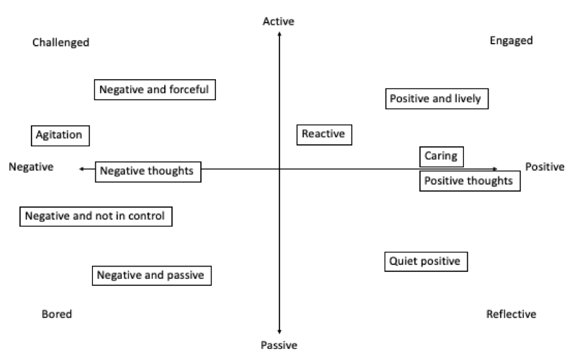
\includegraphics[width=\linewidth]{Fig1.png}
    \caption{Descritores HUMAINE/EARL agrupados com base no Core Affect Model.}
    \label{fig1}
    \source{adaptado a partir de \textcite{russell2003core} por \textcite{rowe2023emotion}.}
    \end{minipage}
\end{figure}

Além desses aspectos, também realizamos a identificação dos alvos das emoções, a fim de definir quais tópicos mobilizaram a expressão das emoções codificadas, tendo em vista que além do tema das mudanças climáticas, outros elementos associados suscitaram expressões emocionais. A identificação desses alvos se mostra como relevante, especialmente, quando se considera o fato de as alterações climáticas estarem envolvidas em um contexto social, histórico e cultural mais amplo, complexificando as suas experiências e expressão de emoções.

\section{Resultados}\label{sec-organizacao}
Considerando a lista dos 56 descritores de emoções apresentadas (\Cref{tbl1}), 20 diferentes emoções foram identificadas neste estudo, as quais tiveram a sua ocorrência em 227 momentos a partir das 197 publicações que constituíram o \textit{corpus} final da pesquisa, uma vez que, em alguns casos, mais de uma emoção foi mobilizada por post. Entre as emoções identificadas, destacaram-se como as mais frequentes a preocupação (n=54), a desaprovação (n=47), o interesse (n=43), a esperança (n=15), dúvida (n=14) e tristeza (n=13). A expressão de outras emoções teve uma menor incidência em termos numéricos (\Cref{fig2}).

A partir da adoção do \textit{Core Affect Model} \cite{russell2003core}, observa-se que a maioria das emoções expressas possui valência negativa (n=139, 61,2\%), em detrimento de expressões emocionais positivas (n=88, 38,8\%), evidenciando modos de enxergar a pauta das mudanças climáticas por um viés que mobiliza problematização ou conflito. Esse aspecto é corroborado pelo fato de que pouco mais da metade das emoções classificadas apresentou alto nível de excitação (116, 51,1\%), sendo 55 ocorrências com valência negativa e 61 com valência positiva. Ao mesmo tempo, um total de 111 expressões de emoções (48,9\%) indicou baixo nível de excitação, correspondendo a 84 ocorrências com valência negativa e 27 com valência positiva.

\begin{figure}[h!]
    \centering
    \begin{minipage}{0.95\linewidth}
    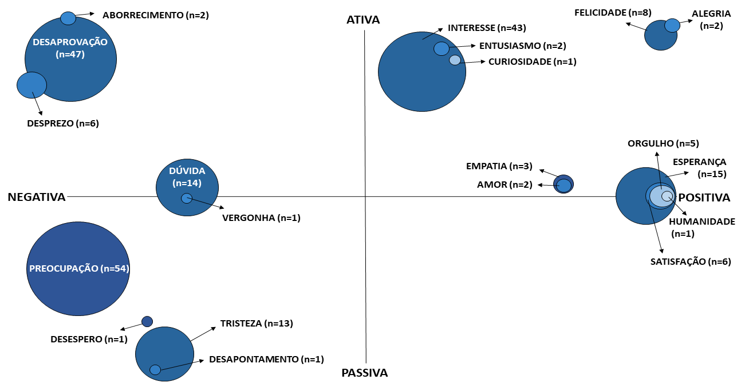
\includegraphics[width=\linewidth]{Fig2.png}
    \caption{Emoções identificadas.}
    \label{fig2}
    \source{Elaborado pelos autores, 2024.}
    \end{minipage}
\end{figure}

\begin{figure}[h!]
    \centering
    \begin{minipage}{0.95\linewidth}
    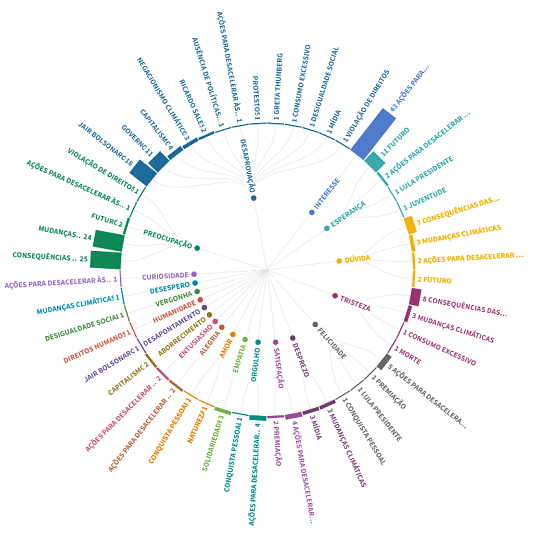
\includegraphics[width=\linewidth]{Fig3.png}
    \caption{Emoções identificadas e respectivos alvos.}
    \label{fig3}
    \source{Elaborado pelos autores, 2024.}
    \end{minipage}
\end{figure}

Embora a maioria das emoções tenha demonstrado um viés negativo, o alvo principal das expressões emocionais foi direcionado às “ações para desacelerar as mudanças climáticas” (n=67), articulado principalmente a partir de emoções como interesse, felicidade e esperança. Na sequência, ainda entre os principais alvos, foram mais frequentes as “consequências das mudanças climáticas” (n=40) e as próprias “mudanças climáticas” (n=35), ambos associados às emoções preocupação, dúvida e tristeza (\Cref{fig3}).

Além dos alvos mencionados, outro tópico associado às mudanças climáticas que suscitou emoções esteve relacionado de forma mais direta a questões políticas e sociais. O ex-presidente do Brasil, Jair Messias Bolsonaro, assim como o seu governo, marcado por ações contrárias aos acordos internacionais do clima, pelo negacionismo climático e desmonte de políticas pró-meio ambiente \cite{fearnside2019retrocessos,miguel2022negacionismo} foram focos da emoção desaprovação (\Cref{fig3}). Na \Cref{tbl2}, apresentamos alguns exemplos de publicações representativas das principais emoções identificadas no \textit{corpus}.

\begin{table}[h!]
\centering
\begin{threeparttable}
\caption{Posts representativos das principais emoções identificadas.}
\begin{small}
\label{tbl2}
\begin{tabular}{p{13cm}}
\toprule
Texto da imagem do post: "MILITANTE CANSADO" "GOVERNO BOLSONARO CORTOU 93\% DA VERBA PARA PESQUISA EM MUDANÇAS CLIMÁTICAS NOS ÚLTIMOS 3 ANOS" Texto da legenda do post: "No meio da \#COP26, com a pressão popular por ações verdadeiramente efetivas contra a crise climática, o governo Bolsonaro tenta mentir na cúpula [DESAPROVAÇÃO], mas os dados revelam. Segundo levantamento da BBC Brasil, pelo Sistema Integrado de Orçamento do Governo Federal (Siop), apenas R\$ 2,1 milhões foram investidos em estudos e projetos para frear as mudanças climáticas nos 3 primeiros anos da gestão ecocida de Bolsonaro [DESAPROVAÇÃO]. O valor é R\$ 29 milhões menor que os investidos entre 2016 e 2018. Desinvestimento em pesquisa ambiental faz parte do projeto de destruição do meio ambiente e entrega dos recursos naturais para o agronegócio. Salles abriu a via para que Joaquim Leite pudesse continuar esse projeto nefasto [DESAPROVAÇÃO]. Só nos resta a luta constante! [ESPERANÇA]" \\ \hline
No futuro só nos restará Brotas!!!! Espia só como Salvador pode ser afetada pelo nível do mar com a alta da temperatura. [PREOCUPAÇÃO] Arrasta pro lado e veja a área do Elevador Lacerda. Essa informação é de uma pesquisa feita pelo Climate Central .
O trabalho publicado na revista Environmental Research Letters identificou as regiões do mundo que podem sofrer inundações "sem precedentes", caso as políticas para combater as mudanças climáticas não sejam colocadas em prática agora pelos países. A matéria completa está no G1/Meio Ambiente. \\ \hline
Legenda do post: "Não podemos mais normalizar tragédias que poderiam ser evitadas! As chuvas intensas em São Paulo já mataram 24 pessoas e desabrigaram 660 famílias. Como moradora da periferia da Zona Sul de São Paulo, minha vida inteira presenciei as consequências ambientais, econômicas e sociais das más políticas públicas urbanas [DESAPROVAÇÃO]. É urgente debatermos meios de reparar financeiramente os mais vulneráveis que já estão sofrendo com a crise climática e adaptar nossas cidades, além de olharmos para o aquecimento global com a prioridade necessária [PREOCUPAÇÃO]. Estou atenta às ações que estão sendo tomadas! Toda a minha solidariedade às vítimas {\Symbola 🙏} [EMPATIA] . . Vídeo @metropoles" \\ \hline
Biodiversidade ameaçada, mudanças climáticas em ritmo acelerado, concentração de gases de efeito estufa, poluição aumentando, desertificação e seca. O cenário é ruim [PREOCUPAÇÃO]. Hoje, Dia Mundial do Combate à Desertificação e à Seca, todos se perguntam como reverter esse quadro. No Plano Conservador da Mantiqueira temos várias frentes de trabalho. Restaurar áreas degradadas, proteger nascentes, cercar florestas, estimular a criação de políticas públicas, promover capacitação e contribuir com a governança local são algumas delas. Atuamos em 425 municípios da região da Mantiqueira e queremos que mais cidades possam unir esforços nessa caminhada  [INTERESSE]. Se você é gestor municipal e ainda não conhece nosso trabalho, entre em contato! Vamos juntos!
\#diadadesertificaçãoedaseca \#desertificação \#seca \#conservaçãoambiental \\ \hline
Ainda há tempo de combater o aquecimento global, ainda há tempo de sonhar e ter esperança [ESPERANÇA], ainda há tempo de resistir e salvar o planeta! Juntos somos muitos {\Symbola ✊📸} @rauldelima \#atopelaterracontraadestruição \\ \hline
Vim puxa um ferro com meu brother [...] e vim sem blusa,hoje Acredito que Sorocaba deve tá mais frio que São Joaquim SC, tava lembrando do pessoal que fala do aquecimento GLOBAL, vocês acreditam nisso mesmo? [DÚVIDA]. \\ \hline
Texto do post: "Triste demais a situação do Rio de Janeiro devido às chuvas torrenciais. Famílias inteiras sendo mortas em mais essa catástrofe [TRISTEZA]. A responsabilidade dos políticos antiecologistas é uma imensa questão diante de mudanças climáticas. Lastimo demais pelo sofrimento da população". Legenda do post: "\#ecologia \#chuvas \#riodejaneiro \#clima" \\ 
\bottomrule
\end{tabular}
\footnotesize {Apesar das publicações transcritas e reproduzidas possuírem um caráter público, por questões éticas, optamos pela não identificação dos seus autores.}
\source{Elaborada pelos autores, 2024.}
\end{small}
\end{threeparttable}
\end{table}

Destarte, se observa que uma diversidade representativa de emoções, valências, níveis de excitação e alvos são apresentados e se articulam de diferentes formas em torno da questão das mudanças climáticas nos conteúdos publicados no Instagram, evidenciando a complexidade do assunto e a necessidade de aprofundamento acerca de sua compreensão.

\section{Discussão}\label{sec-organizacao-latex}
Considerando os resultados apresentados, observamos a prevalência de emoções negativas em relação às mudanças climáticas nos conteúdos da rede social Instagram entre os anos de 2021 e 2022 no Brasil, tomando como base o \textit{corpus} investigado. Preocupação (n=54) e desaprovação (n=47) foram as emoções mais evocadas, indicando um viés particular de perceber o fenômeno em pauta. Nesse contexto, o Instagram foi evidenciado não apenas como uma plataforma voltada para a produção e compartilhamento de fotos e vídeos de entretenimento, comumente apontada em outros estudos por meio de uma perspectiva alicerçada em um tom emocional predominantemente positivo \cite{sonne2018expression}, sendo, também, palco para emoções negativas.

Emoções positivas, como interesse (n=43), esperança (n=15), entre outras, mesmo que em um menor número, também foram expressas (\Cref{fig2}), complexificando os modos de compreensão acerca das mudanças climáticas. Acerca das emoções mobilizadas, importa refletir sobre os seus alvos, quando se percebe que apesar de classificadas como de valência negativa, algumas das emoções apontam para um viés de implicação, atenção e comprometimento em torno das mudanças climáticas. A preocupação, por exemplo, foi mobilizada especialmente em relação às “consequências das mudanças climáticas”, “mudanças climáticas”, “futuro” e “ações para desacelerar as mudanças climáticas”. Nesse sentido, podendo ser entendida como ligada aos processos cognitivos voltados para a resolução de problemas e a autorregulação, possuindo um caráter adaptativo com vistas a reduzir potenciais ameaças \cite{watkins2008repetitive}, a preocupação em relação às mudanças climáticas, mesmo que possua uma expressão negativa, também aponta para a perspectiva de um olhar que busca lidar com os acontecimentos que a agenciam, a fim de evitar potenciais riscos.

Aspecto semelhante pode ser problematizado em relação à desaprovação, emoção evocada no \textit{corpus} a partir de focos relacionados, sobretudo, ao ex-presidente do Brasil, Bolsonaro, e às ações de seu governo, especialmente diante da adoção de posições contrárias às políticas voltadas para o meio ambiente e a desaceleração das mudanças climáticas, tendo em vista uma atuação pautada pelo negacionismo climático \cite{fearnside2019retrocessos,miguel2022negacionismo}. Ao desaprovar as ações dos atores citados, nota-se a partir dos conteúdos examinados uma perspectiva voltada para o cuidado e preservação do meio ambiente. Desse modo, a desaprovação, apesar de negativa, pode ser lida como uma expressão positiva em se tratando da oposição a posturas que tendem a asseverar as mudanças climáticas. Em outros estudos acerca da temática, no caso, com foco nos conteúdos brasileiros no TikTok, Bolsonaro foi também criticado pela sua conduta e responsabilizado acerca das consequências advindas das alterações no clima \cite{evangelista2024narrativas}.

A recorrência de emoções negativas sobre a pauta relativa ao clima corrobora com os achados de outros estudos, como os de \textcite{cody2015climate,flores2018emociones}. Entretanto, salienta-se a necessidade de refletir sobre a complexidade inerente à expressão das emoções. Isso porque algumas emoções, apesar de serem socialmente percebidas como negativas, possuem importância em termos de experiência e aquisição de conhecimento para lidar com os acontecimentos. Algumas pesquisas do campo da psicologia vêm, inclusive, atentando para estes aspectos, como as desenvolvidas por \textcite{parrott2014positive,niehoff2020curiosity}. As emoções negativas, para esses autores, possuem uma função adaptativa de proteção e sobrevivência, no sentido de que podem fornecer aos sujeitos oportunidades de adquirir conhecimentos, antecipar-se e reduzir incertezas.

Além de se problematizar a ocorrência dessas emoções negativas, identificadas entre as mais frequentes, cabe refletir também sobre as emoções positivas que emergiram no \textit{corpus}, sendo mais recorrentes o interesse e a esperança. Ambas as emoções apontam para conteúdos que evidenciam um envolvimento dos produtores das publicações com a causa do meio ambiente, demonstrando interesse em ações que possam dirimir as mudanças climáticas e os seus efeitos, assim como a esperança no futuro. Tais achados são semelhantes ao da pesquisa de \textcite{balbe2017twitter}, que evidenciaram, a partir da análise de um \textit{corpus} do Twitter (atual X), expectativas positivas em relação ao estabelecimento de acordos internacionais em defesa do clima.

Articuladas, as emoções destacadas explicitam o quanto as mudanças climáticas têm sido tomadas como focos de interesse, atenção e mobilizadoras de expressões emocionais, que em sua diversidade, ilustram a complexidade demandada tanto em se tratando do assunto, como das percepções, atitudes e interesses evocados em torno dele por parte dos sujeitos e dos conteúdos produzidos nas redes sociais.

\section{Considerações finais}\label{sec-idioma}
Tivemos como objetivo, neste estudo, identificar e analisar as emoções expressas em torno da questão das mudanças climáticas a partir de conteúdos públicos produzidos na rede social Instagram entre os anos de 2021 e 2022, tendo como base o contexto brasileiro. Entre os resultados, foi observado a prevalência de emoções negativas sobre o assunto, com ênfase para a preocupação e desaprovação, corroborando com outros estudos anteriores. Ao mesmo tempo, entre as emoções positivas, apesar de possuírem menor incidência, se destacaram o interesse e a esperança.

Apesar da maior frequência de emoções negativas em relação ao \textit{corpus} investigado, as análises apontam para a necessidade de se refletir sobre a complexidade das emoções evocadas, assim como sobre os seus respectivos alvos. Tal perspectiva é reforçada quando se percebe que emoções negativas, como preocupação e desaprovação não apontam, necessariamente, para um sentido de recusa ou negação das mudanças climáticas, mas de envolvimento e implicação, o que pode ser avaliado como expressões emocionais favoráveis à discussão, o que também é proposto por investigações mais recentes sobre o lado positivo das emoções negativas.

Dessa forma, as emoções negativas, articuladas às emoções positivas, ratificam a atenção e sentido de cuidado proposto pelos conteúdos das publicações no que concerne às mudanças climáticas. Ressalta-se que esses resultados são correspondentes a um recorte específico. Assim, sugere-se a promoção de outras investigações semelhantes a partir de outras redes sociais e temporalidades, a fim de ampliar as discussões produzidas, especialmente, se considerando o crescimento dos debates sobre as mudanças climáticas, haja vista a maior ocorrência de seus efeitos.



\section{Agradecimentos}\label{sec-resumo}
Este artigo foi realizado no escopo do Instituto Nacional de Comunicação Pública da Ciência e Tecnologia, que conta com financiamento do Conselho Nacional de Desenvolvimento Científico e Tecnológico [CNPq, 465658/2014-8] e Fundação Carlos Chagas Filho de Amparo à Pesquisa do Estado do Rio de Janeiro [FAPERJ, E-26/200.89972018]. O estudo também se insere no projeto apoiado pelo Edital Universal Chamada CNPq/MCTI Nº 10/2023 - Faixa B - Grupos Consolidados, 401881/2023-7] e pela chamada Projeto em cooperação com comprovada articulação internacional [CNPq, 441083/2023-4], liderados por Luisa Massarani. Luisa Massarani agradece ao CNPq pela Bolsa de Produtividade 2 e 1B. Luisa Massarani e Thaiane Oliveira agradecem à Faperj pela bolsa Jovem Cientista do Nosso Estado e Cientista do Nosso Estado.


\printbibliography\label{sec-bib}
% if the text is not in Portuguese, it might be necessary to use the code below instead to print the correct ABNT abbreviations [s.n.], [s.l.]
%\begin{portuguese}
%\printbibliography[title={Bibliography}]
%\end{portuguese}


%full list: conceptualization,datacuration,formalanalysis,funding,investigation,methodology,projadm,resources,software,supervision,validation,visualization,writing,review
\begin{contributors}[sec-contributors]
\authorcontribution{Geilson Fernandes de Oliveira}[datacuration,formalanalysis,investigation,methodology,validation,visualization,writing,review]
\authorcontribution{Luisa Massarani}[conceptualization,formalanalysis,funding,investigation,methodology,projadm,resources,validation,supervision,writing,review]
\authorcontribution{Graziele Scalfi}[datacuration,formalanalysis,investigation,methodology,validation,writing,review]
\authorcontribution{Marcelo Alves dos Santos Junior}[datacuration,formalanalysis,investigation,methodology,resources,software,validation,writing,review]
\authorcontribution{Thaiane Oliveira}[formalanalysis,funding,investigation,methodology,resources,software,validation,writing,review]
\end{contributors}


\end{document}

